\chapter{Experimental procedure}
This chapter consists of the experimental setup and measurement procedure. Firstly the required apparatus is specified. After the apparatus is known, the calibration of the magnetic field is explained. At last the measurement procedure for the Hall voltage is discussed.

\section{Experimental setup}
The experimental setup can be divided into two sections. The first section is used to create a magnetic field. A schematic of this part of the experimental setup is shown in Figure \ref{fig:schematic_setup_magnets}. The maximum continues current supported by the coils is 5 A, this current is supplied by the power supply unit (PSU). It is possible to supply the coils with a higher current, for example 15 A. However, this has to be in a relatively short time frame. This is so the coils do not get damaged. A list of the required apparatus is shown in Figure \ref{fig:apparatus}, which can be found in Appendix-A. The power supply used to power the coils has to be able to deliver a current up to 5 A. This current is measured with a TTi 1604 digital multimeter. This multimeter is used for all current and voltage measurements. The necessary magnetic field strength to be created is between 0.1 and 0.6 T \cite{apparatus_silver}.\\
    \begin{figure}[!htbp]
    \begin{center}
        \begin{minipage}[t]{0.45\textwidth}
            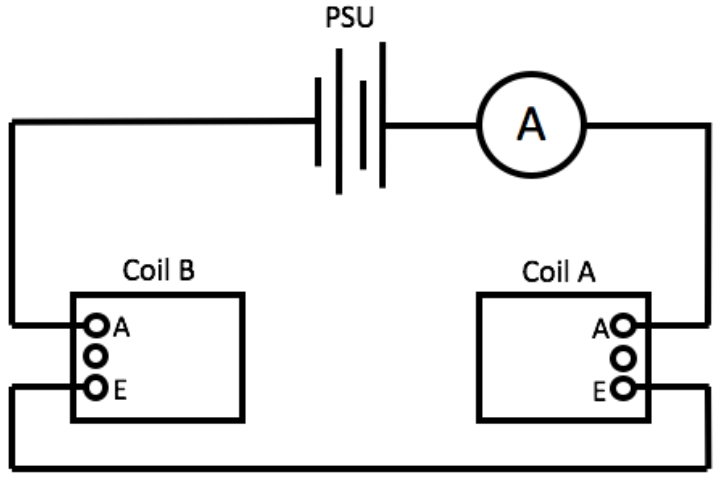
\includegraphics[scale=0.35]{figuren/schematic_setup_magnets.png}
            \caption{A schematic of the coil configuration.} \label{fig:schematic_setup_magnets}
        \end{minipage}
        \begin{minipage}[t]{0.45\textwidth}
            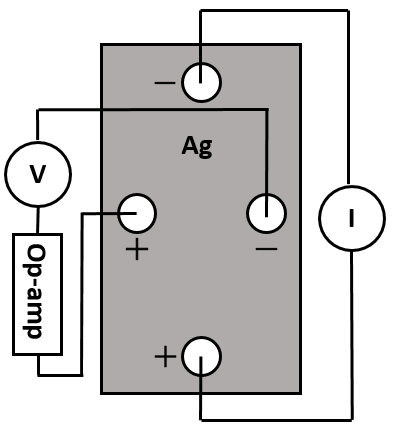
\includegraphics[scale=0.5]{figuren/schematic_hall_voltage.png}
             \caption{The schematic setup for the experimental setup of the Hall effect.}\label{fig:schematic_hall_effect}
        \end{minipage}
    \end{center}
    \end{figure}
The second section of the experimental setup consists of the material on which the Hall voltage is measured. A schematic of this part of the experimental setup can be seen in Figure \ref{fig:schematic_hall_effect}. The PSU which supplies the current through the material must be able to supply up to 20 A. The Hall voltage is measured by a multimeter. An operational amplifier (Op-amp) might be needed to amplify the Hall voltage. The need for an Op-amp depends on the material used. Silver for example, has a Hall voltage of 5 $\mu$V when a current of 15 A flows through the material, in a 0,2 T magnetic field perpendicular to the flow of current \cite{halleffectzilver}. 5 $\mu$V cannot be measured by the TTi 1604 multimeter, therefor an Op-amp circuit is required to amplify the voltage to an order of magnitude which can be measured by the TTi 1604 \cite{dmm}. The chosen Op-amp is an AD521, which can amplify the signal up to one thousand times. With a maximum output voltage of 30 V \cite{AD521}. Note that the exact amplification of the Op-amp has to be determined before it is used in a measurement. This can be done by using two multimeters and a signal generator to apply a known signal and measure the Op-amps output. At last a computer with CASSY Lab is required for the data-acquisition of the Combi B-Sensor S. The Combi B-Sensor S measures the strength of the magnetic field at the Hall apparatus center with respect to earth's magnetic field.
    
\section{Magnetic field calibration}
The magnetic field strength created by the coils as a function of the current through them has to be known. This is due to the fact the magnetic field strength sensor does not fit in between the coils while the Hall apparatus is present. By experimenting it can be seen that the magnetic field in between the coils is homogeneous. For this reason a model for the magnetic field as function of current through the coils can respectively simply be made. This part of the experimental setup can be seen in Figure \ref{fig:cal_setup}.\\
    \begin{figure}[!htbp]
    \begin{center}
        \begin{minipage}[t]{0.45\textwidth}
            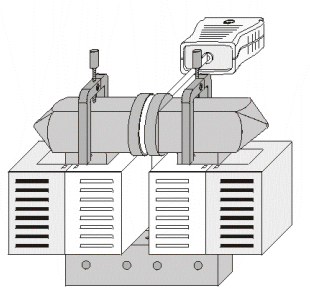
\includegraphics[scale=0.8]{figuren/schematic_calibration.png}
            \caption{Calibration of the magnetic field \\ schematically  \cite{halleffectzilver}.}\label{fig:cal_setup}
        \end{minipage}
        \begin{minipage}[t]{0.45\textwidth}
            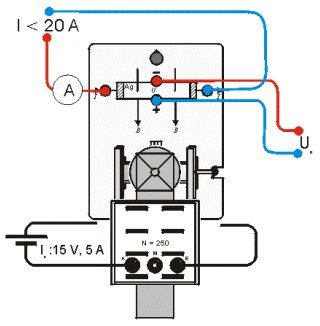
\includegraphics[scale=0.8]{figuren/experimental_setup.png}
            \caption{The wiring diagram for the experimental setup of the Hall effect \cite{halleffectzilver}.}\label{fig:experimental_setup}
        \end{minipage}
    \end{center}
\end{figure}
The magnetic field as a function of the amount of current through the coils is calibrated as follows. The current through the coils is increased by steps of 0,1 A from 0 to 5 A. At each step the strength of the magnetic field is measured. This data can be used to create a mathematical model, which later on can be used to calculate the magnetic field strength when the current through the coils is known. This is done in Chapter 4.1. It is important to emphasize that the hysteresis characteristics of the soft metal surrounded by the coils is ignored due to simplicity.

\section{Hall voltage measurement}
The experimental setup should look like Figure \ref{fig:experimental_setup} when the coils and Hall apparatus are setup according to respectively Figure \ref{fig:schematic_setup_magnets} and Figure \ref{fig:schematic_hall_effect}. A Hall voltage can be create by two physical situations. When the current flow in the material is constant, the strength of the magnetic field perpendicular to this current flow has to increase. Or when the strength of the magnetic field is constant, the current has to increase. Either one will create a Hall voltage, as long as Equation \ref{eq:Hall Voltage2} is not equal to zero. Which means that $B$ and $I$ have to be larger then 0. \\
In case of the current through the coils being a constant, the magnetic field strength perpendicular to the material has to be increased. This is done by starting with 0 A through the coils, going up all the way to 5 A in steps of 0,5 A. This way the magnetic field $B$ can be calculated because the current through the coils is known, the Hall voltage at this specific magnetic field strength can also be measured. This should result in a linear model, since Equation \ref{eq:Hall Voltage2} is linear. \\
The same thing goes for a constant magnetic field strength of for example 0,2 T. The current through the material is varied from 0 to 20 A in steps of 1 A. This should also result in a linear model because of the reason stated above. \\
In this experiment a Hall apparatus with silver has been used in a 0,3 T magnetic field. It it important to note that two different silver apparatuses have been used with part number '58681 B2' \& '58681'. Why this is important will become clear in Chapter 6. When measuring the hall voltage, the offset voltage has to be determined first. This is done by turning off the magnetic field and measuring the offset voltage across the Hall apparatus. Once this is done the magnetic field can be turned on, which will result in a voltage increase due to the Hall effect. The actual difference between the measured voltage with magnetic field and the offset voltage is the voltage due to the Hall effect. One can also reverse the magnetic field to remove any longitudinal impurities in the force vector on the charge carriers.

\section{Python simulation}
Equation \ref{eq:Hall Voltage2} can be used to simulate experimental results. These simulations can be used to verify the actual experimental results while measuring.
    \begin{equation}
        U_H = \frac{1}{n \cdot e} \frac{B \cdot I}{d} \tag{\ref{eq:Hall Voltage2}}
    \end{equation}
Multiple physical situations have been modelled. In each situation all variables except for one, have been kept constant. These situations give insight in how the Hall voltage changes for different materials in different situations. In each situation Equation \ref{eq:e} has been used as the value for the elementary charge $e$.